% Permission is granted to copy, distribute and/or modify this document
% under the terms of the GNU Free Documentation License, Version 1.2
% or any later version published by the Free Software Foundation;
% with no Invariant Sections, no Front-Cover Texts, and no Back-Cover
% Texts.  A copy of the license is included in the section entitled "GNU
% Free Documentation License".
% Copyright 2014 EDF
%

%%%%%%%%%%%%%%%%%%%%%%%%%%%%%%%%%%%%%%%%%%%%%%%%%%%%%%%%%%%%%%%%%%%%%%%%%%%%%%%%%%%%%%%%%%
\section{Architecture guide}

This document makes up the general specification design for the architecture of the OTLHS module.
Several classes implement the \textit{pimpl} idiom (pointer to implementation) to hide implementation
details.

\subsection{SpaceFilling}

\begin{figure}[htb]
  \begin{center}
    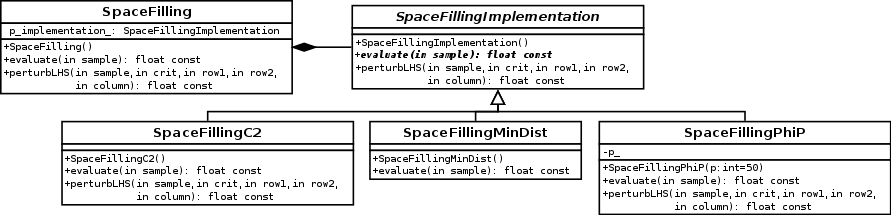
\includegraphics[scale=0.5]{SpaceFilling.png}
    \caption{SpaceFilling classes}\label{fig:archi:space-filling}
  \end{center}
\end{figure}

These classes implement different space filling criteria, which are consumed by
\texttt{OptimalLHS} algorithms.

\subsection{OptimalLHS}

\begin{figure}[htb]
  \begin{center}
    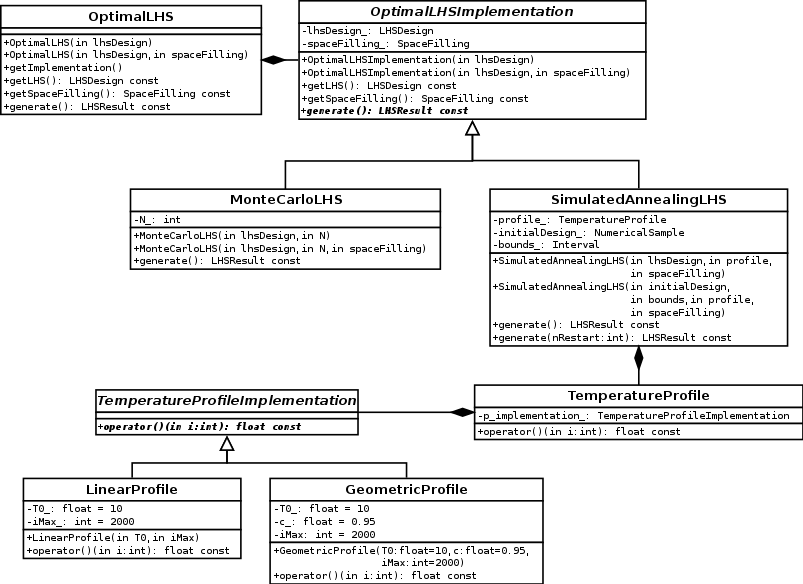
\includegraphics[scale=0.5]{OptimalLHS.png}
    \caption{OptimalLHS classes}\label{fig:archi:optimal-lhs}
  \end{center}
\end{figure}

This is the main class hierarchy.  The \texttt{OptimalLHS} class is an abstract class,
inherited by \texttt{MonteCarloLHS} and \texttt{SimulatedAnnealingLHS}.  They implement the
\texttt{generate} method, which returns an \texttt{LHSResult} instance.

\subsection{LHSResult}

\begin{figure}[htb]
  \begin{center}
    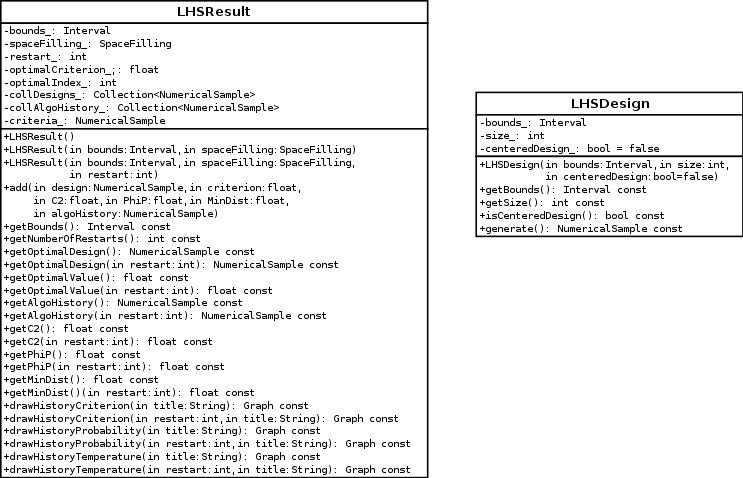
\includegraphics[scale=0.65]{LHSResult.png}
    \caption{LHSDesign and LHSResult classes}\label{fig:archi:lhs}
  \end{center}
\end{figure}

As OpenTURNS already provides an \texttt{LHS} class, we had to rename it into \texttt{LHSDesign}.
Its constructor takes as arguments variable bounds, the size of the generated sample, and an optional
boolean parameter to tell whether randomized (default) or centered LHS have to be generated.

The \texttt{LHSResult} class is returned by \texttt{OptimalLHS.generate()} and contains algorithm
results.  The \texttt{add} method is called by \texttt{OptimalLHS} (once if there is no restart,
and one plus one by restart otherwise), and informations can then be extracted by accessors.
If no restart argument is specified, informations about global optimum are retrieved.  If a
restart number is provided, informations about this specific run are retrieved.


